% This is samplepaper.tex, a sample chapter demonstrating the
% LLNCS macro package for Springer Computer Science proceedings;
% Version 2.20 of 2017/10/04
%
\documentclass[runningheads]{llncs}
%
\usepackage{graphicx}
\usepackage{subfig}

% For todo notes (workaround for 2-column using marginnote from: https://tex.stackexchange.com/questions/52680/how-can-i-make-todo-comments-when-using-the-multicol-package)
\usepackage[textsize=tiny, textwidth=2.0cm]{todonotes}


\begin{document}
%
\title{State Estimation and Data Assimilation for an Agent-Based Model using a Probabilistic Framework 
\thanks{This work was supported by a European Research Council (ERC) Starting Grant [number 757455], a UK Economic and Social Research Council (ESRC) Future Research Leaders grant [number ES/L009900/1], an ESRC-Alan Turing Fellowship [ES/R007918/1] and through an internship funded by Improbable (\url{https://improbable.io/}).}}

%
\titlerunning{Probabilistic estimation of ABMs}
% If the paper title is too long for the running head, you can set
% an abbreviated paper title here
%

\author{Nick Malleson\inst{1,3}\orcidID{0000-0002-6977-0615} \and
Luke Archer\inst{3} \and
Minh Kieu\inst{1,3}\orcidID{0000-0001-7798-6195} \and
Jonathan A. Ward\inst{2}\orcidID{0000-0003-3726-9217} \and
Alison Heppenstall\inst{1,3}\orcidID{0000-0002-0663-3437} \and
Christoforos Anagnostopoulos\inst{4}
}
%

\authorrunning{Malleson et al.}
% First names are abbreviated in the running head.
% If there are more than two authors, 'et al.' is used.
%
\institute{
School of Geography, University of Leeds, LS2 9JT, UK \\
\url{http://geog.leeds.ac.uk/} \\
 \and
School of Mathematics, University of Leeds, LS2 9JT, UK \\
\url{http://maths.leeds.ac.uk} 
\and
Leeds Institute for Data Analytics (LIDA), University of Leeds, LS2 9JT, UK \\
\url{http://lida.leeds.ac.uk} 
\and
Improbable, 10 Bishops Square, London, E1 6EG \\
\url{http://www.improbable.io}
}
%
\maketitle              % typeset the header of the contribution
%
\begin{abstract}

This paper outlines a framework for state estimation and data assimilation in agent-based models, using a Bayesian probabilistic framework. It presents initial attempts to begin to quantify the type and volume of data that would be required to realistically model a crowd of people in real time.  It contributes to the challenge set out in the workshop theme in two ways. Firstly, by developing methods that support ``trusted models that can be used by industry and governments to enhance decision-making, and that can incorporate real (and real-time) data sets in a meaningful way''. Secondly, regarding the `humans and devices' theme specifically, by beginning to estimate the volume of sensors that would be required in order to successfully model crowds in real time. Without a reliable means of incorporating real-time data into urban models, their use will continue to be limited to scenario evaluation based on historical data rather than providing the most likely estimates of the \textit{current} state of urban systems as well as short-term forecasts.

\keywords{Agent-based modelling \and Probabilistic programming \and Uncertainty \and Data assimilation \and State estimation \and Bayesian inference }
\end{abstract}
%
%
%
 
\newpage
\pagenumbering{arabic} % Reset the page number as everything up to now was a title & abstract
\setcounter{footnote}{0} % same for footnote counter

%
%
% ***************** Introduction *****************
%
%

\section{Introduction and Objectives}

Calibration -- the process of finding optimal values for a model's parameters -- is reasonably well studied in the field of agent-based modelling. Two aligned topics that are much less well studied, however, are those of \textit{state estimation} and \textit{data assimilation}. State estimation refers to the practice of estimating the \textit{true} state of a system. Although their complexity precludes the true state of human systems ever being known precisely, it can be estimated by combining a model of the system with observations (data). The practice of estimating a system's \textit{current} (i.e. real-time) state using a model and some data is often termed data assimilation\footnote{It is worth noting that although data assimilation techniques can be used to adjust model parameters in response to new data, here the technique is applied solely to the task of state estimation.}.  Data assimilation has, and continues to be, extremely well studied in fields such as meteorology~\cite{kalnay_atmospheric_2003} where it has been credited as being part of the reason that weather forecasts have improved so substantially in recent years~\cite{bauer_quiet_2015}. 

Applications of data assimilation in agent-based modelling are scarce, however; only a handful of attempts have been published~\cite{malleson_understanding_2018,wang_data_2015,ward_dynamic_2016}. The aim of this research is to contribute to this emerging field by performing data assimilation on a simple agent-based model of a hypothetical crowd. The work builds on previous work that was originally presented at ABMUS 2018~\cite{malleson_understanding_2018}. A series of `identical twin' experiments are planned, whereby the agent-based model first generates `pseudo-truth' data that reflect the `true' state of the system (in the real world such data are never available) and then the model is re-run in a data assimilation framework that attempts to replicate the truth data. Importantly, by varying the amount of information about the true system state that is provided to the data assimilation algorithm it is possible to estimate the amount of information that might be required were a real crowd of people to be simulated. Here it will be assumed that some individuals in the hypothetical data are tracked, so their spatio-temporal locations are known, but in future work the framework will be extended to aggregate data as well (i.e. counts of people rather than individual traces). As discussed shortly, the paper also makes use of a relatively novel computational approach: probabilistic programming. Hence the contributions of this paper are two-fold, it:

\begin{enumerate}
	\item provides a framework to estimate the volume of data that are necessary to simulate a crowd in real-time;
	\item explores the value of the probabilistic approach to modelling as a means of performing data assimilation on an agent-based model.
\end{enumerate}

Experimental results are not yet available, but are under preparation and will be available for the workshop.



%
%
% ***************** StationSim *****************
%
%
\section{An Example Agent-Based Model: \textit{StationSim}}

$ $ % (this is because a \todo straight after a \section confuses latex)

The hypothetical model used here is a simple system of pedestrians, each of whom move from an entrance towards one of two exits. The model environment is illustrated in Figure~\ref{fig:pedestrian_model_environment}. It has been designed to be as simple as possible and yet meet two criteria:

\begin{enumerate}
	\item be loosely representative of a spatial human system (in this case the model represents an abstract train station, where passengers arrive on a train and need to cross the station concourse to leave through the exits);
	\item exhibit emergence (in this case emergence takes the forms of \textit{crowding} that occurs as a result of the random distributions of agents who all have different maximum walking speeds).
\end{enumerate}

\begin{figure}
	\centering
	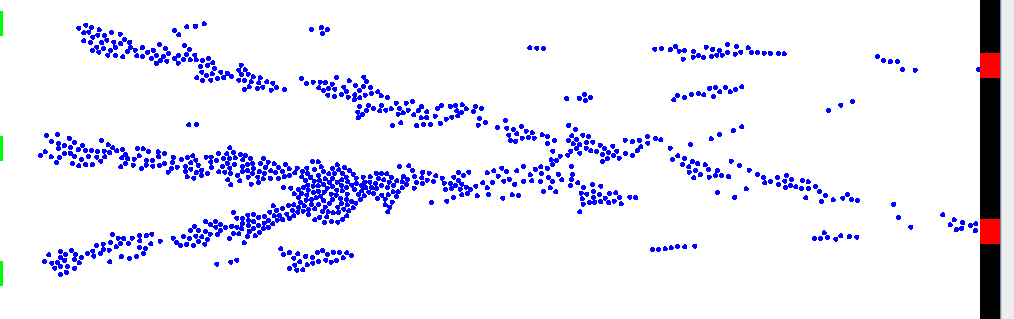
\includegraphics[width=0.9\textwidth]{figures/pedestrian_model_environment2}
	\caption{A snapshot of the simple, hypothetical model that is used here. Agents move from left to right.} \label{fig:pedestrian_model_environment}
\end{figure}

The model is Markovian, such that it can produce  output from a set of inputs (here termed the `state vector') without any other information. The \textit{state vector}, at a time $t$, contains all of the agent ($i = \{ 0, 1, \dots, N \} $) variables ($\overrightarrow{v_i}$) but not any model parameters. Therefore 
\begin{equation}
S_t  = \left[ \begin{array}{cccc}
\overrightarrow{v_0} &  \overrightarrow{v_1} &  \dots & \overrightarrow{v_N} 
\end{array} \right]
\end{equation} 
where $\overrightarrow{v_i}$ represents the $x$ and $y$ coordinates\footnote{Note that the \textit{current} speed of an  agent need not be included in the state vector because it is a deterministic function of an agent's maximum speed and the positions of the other agents.} of the each agent ($i$) at time $t$:
\begin{equation}
\overrightarrow{v_{i,t}}  = \left[ \begin{array}{cc} x_{i,t} & y_{i,t} \end{array}  \right]
\end{equation}

There are numerous model and agent parameters -- such as the destination exit and maximum speed for each agent -- but these are kept constant throughout the experiments and so need not be included in the state vector. It would be possible to include these parameters in the state vector and estimate them along with the variables, but this will be tested in future work.

%
%
% ***************** Modelling *****************
%
%
\section{Modelling Framework}

We take a Bayesian approach to data assimilation. As Figure~\ref{fig:da_framework} illustrates, the prior estimate of the state of the (pseudo\footnote{Recall that, in this case, the `real' system is actually a single run of the model as per the `digital twin` experimental framework.}) real system is generated by running the agent-based model forward from the last point in time that historical observational data were available ($t-1$ in Figure~\ref{fig:da_framework}). The prior provides uncertain estimates of the current system state, represented in the form of a distribution over the state vector ($S$). At time $t$ (i.e. `now'), it is hypothesised that new data have arrived and these need to be assimilated into the model. At present, the locations of all agents in the pseudo-truth are observed, which is analogous to every person in the station having their positions tracked. Although some noise is added to the observations, this is still more data than would usually be available in the real world and later experiments (discussed shortly) will reduce the amount of information provided. 

To incorporate the new observations a Bayesian network (a probabilistic graphical model) is constructed that represents the relationships between the different elements of the state vector (the $x$ and $y$ coordinates for all agents) and the station model itself. In effect, each element in the state vector becomes a vertex in the graph, along with the station model. 

\begin{figure}
	\centering
	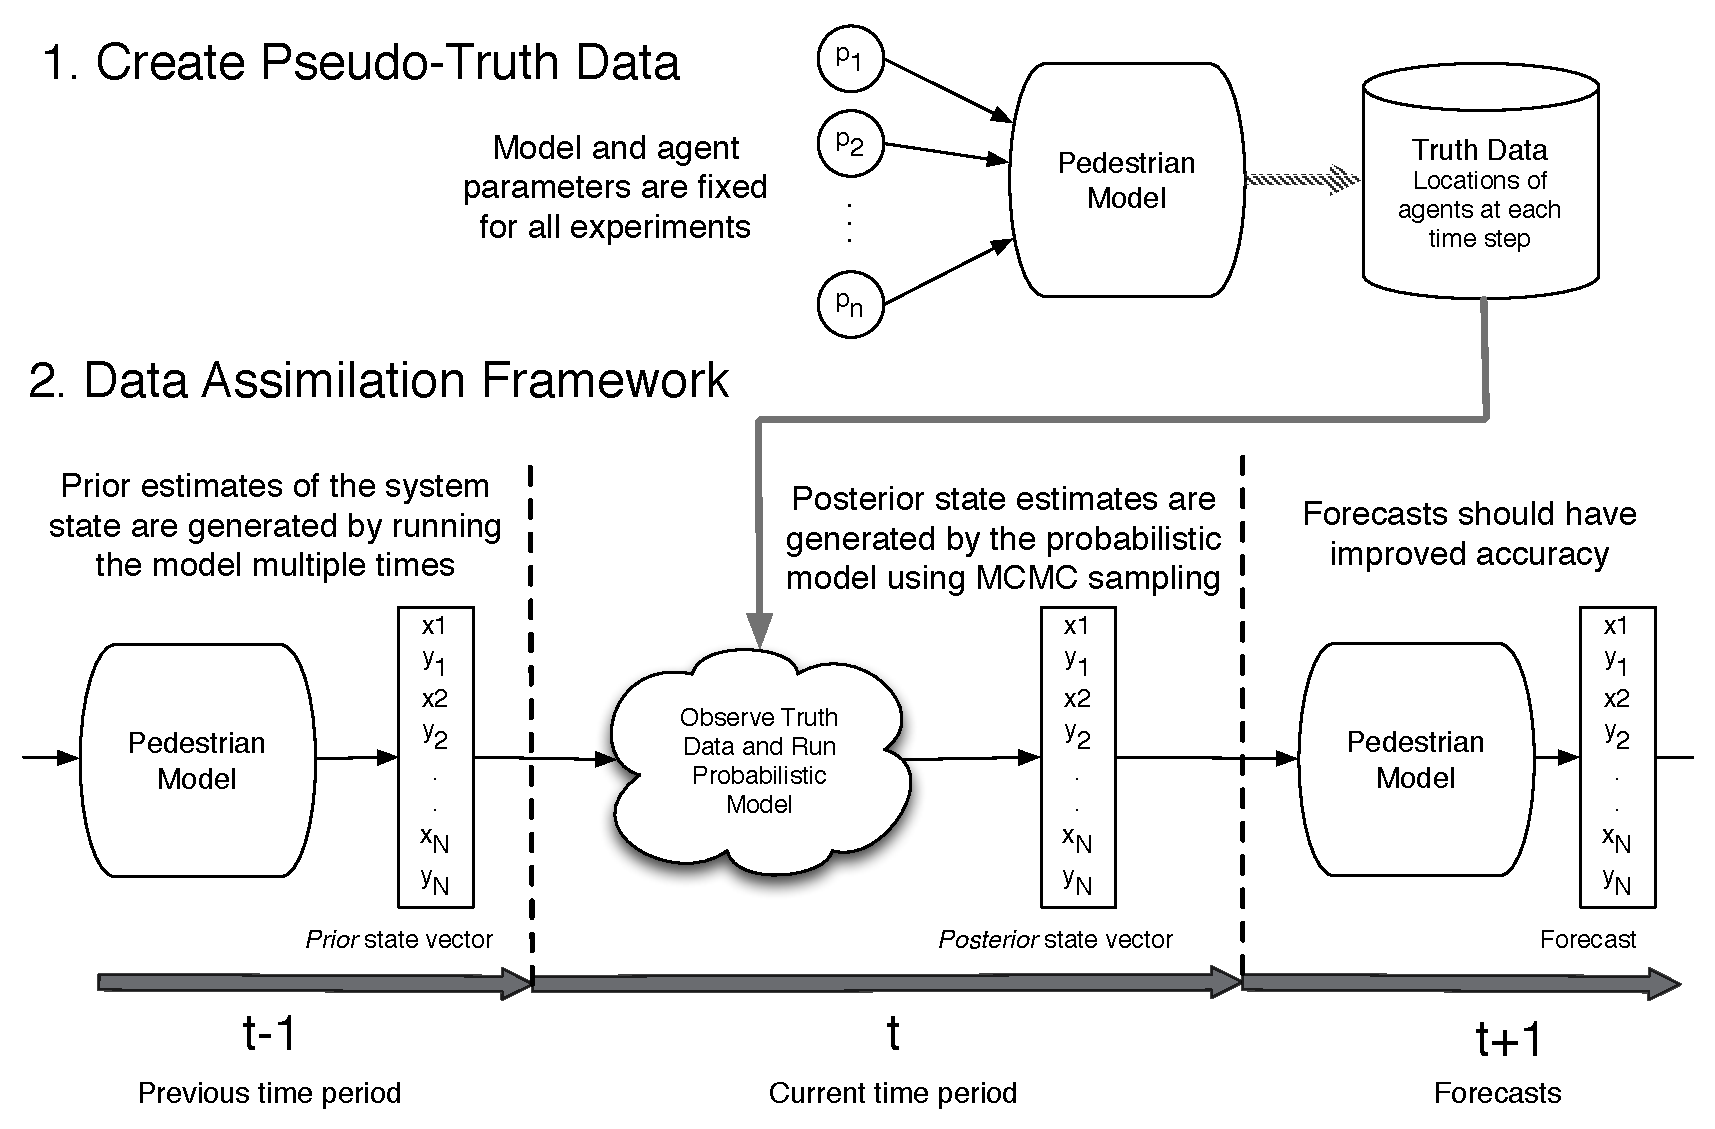
\includegraphics[width=0.9\textwidth]{figures/da_framework}
	\caption{The framework for conducting state estimation and data assimilation using the identical twin experiment and a probabilistic model. This builds on the initial work outlined in \cite{malleson_understanding_2018}.} \label{fig:da_framework}
\end{figure}


Then, through Markov chain Monte Carlo (MCMC) sampling, posterior estimates of the state vector are produced.  Hence the posterior is the new estimate of the system state that is obtained once the most recent observations from the (pseudo) real system have been incorporated. This is useful in itself as it potentially provides a more up-to-date estimate of the current state of the system. In addition, these posterior estimates can then be re-inserted as the new priors to run new model forecasts (i.e. $t+1$ in Figure~\ref{fig:da_framework}). As the new forecasts take the most recent available data into account they should be more accurate than forecasts made from earlier, out-of-date data. Here, the whole process is repeated a number of times to reflect the real practice of data assimilation that might take place were a model really attempting to simulate a system in real time.

\section{Probabilistic Programming and the Bayesian network}

This framework lends itself extremely well to the relatively new approach of `probabilistic programming'~\cite{ghahramani_bayesian_2012,ghahramani_probabilistic_2015}. This is a structure for writing computer programs whereby variables represent probability distributions (i.e. random variables) rather than single values. This approach is therefore ideally suited to Bayesian modelling. Here, a new probabilistic programming library, \textit{keanu}\footnote{Keanu: \url{https://github.com/improbable-research/keanu}}, is used. Keanu provides the functionality required to create a Bayesian network and perform MCMC sampling to generate the posterior estimates. 

Importantly, the Bayesian network is agnostic to the type of information that the nodes in the graph represent. At present, the nodes represent the individual elements of the state vector (i.e. individual agent locations) and observations from the pseudo-truth model map directly onto these nodes. As mentioned above, this is analogous to tracking each individual. However, an alternative approach would be to assume that the individual positions cannot be directly observed, and instead additional random variables can be defined that are functions of those states and which \textit{can} be observed. For example, the aggregate spatial distributions of agents could be used. The probabilistic model is not challenged by this formulation, since it is perfectly capable of producing posteriors over all nodes, regardless of whether they are observable or latent. This is much closer to a realistic application (e.g. by collecting aggregate crowd density data rather than tracking individuals) and, through the Bayesian network, an elegant way of incorporating different types of data. 


\section{Proposed Experiments and Expected Results} 

At the time of writing the experiments are under way. By the time of the workshop the paper will report initial experiments that explore: the ability of the framework to realistically model the true system state with full (albeit noisy) information about every agent; the impacts of reducing the number of observed agents (i.e. only observing a portion of the state vector); observing aggregate rather than individual-level data (i.e. all agent locations are latent).




\newpage
\pagenumbering{gobble} % turn off page numbering
\bibliographystyle{splncs04}
\bibliography{2019-ABMUS-KeanuProbabilistic}

\end{document}
